\newpage

\section{Probabilité conditionnelle}

\begin{intuitionbox}[Question Fondamentale]
La probabilité conditionnelle est le concept qui répond à la question fondamentale : comment devons-nous mettre à jour nos croyances à la lumière des nouvelles informations que nous observons ?
\end{intuitionbox}

\subsection{Définition de la Probabilité Conditionnelle}

\begin{definitionbox}[Probabilité Conditionnelle]
Si $A$ et $B$ sont deux événements avec $P(B) > 0$, alors la probabilité conditionnelle de $A$ sachant $B$, notée $P(A|B)$, est définie comme :
$$P(A|B) = \frac{P(A \cap B)}{P(B)}$$
\end{definitionbox}

\begin{intuitionbox}
Imaginez que l'ensemble de tous les résultats possibles est un grand terrain. Savoir que l'événement $B$ s'est produit, c'est comme si on vous disait que le résultat se trouve dans une zone spécifique de ce terrain. La probabilité conditionnelle $P(A|B)$ ne s'intéresse plus au terrain entier, mais seulement à la proportion de la zone $B$ qui est également occupée par $A$. On "zoome" sur le monde où $B$ est vrai, et on recalcule les probabilités dans ce nouveau monde plus petit.
\end{intuitionbox}

\subsection{Règle du Produit (Intersection de deux événements)}

\begin{theorembox}[Probabilité de l'intersection de deux événements]
Pour tous événements $A$ et $B$ avec des probabilités positives, nous avons :
$$P(A \cap B) = P(A)P(B|A) = P(B)P(A|B)$$
Cela découle directement de la définition de la probabilité conditionnelle.
\end{theorembox}

\begin{intuitionbox}
Pour que deux événements se produisent, le premier doit se produire, PUIS le second doit se produire, sachant que le premier a eu lieu. Cette formule exprime mathématiquement cette idée séquentielle.
\end{intuitionbox}

\begin{examplebox}
Quelle est la probabilité de tirer deux As d'un jeu de 52 cartes sans remise ?
Soit $A$ l'événement "le premier tirage est un As", avec $P(A) = \frac{4}{52}$. Soit $B$ l'événement "le deuxième tirage est un As". Nous cherchons $P(A \cap B)$, que l'on calcule avec la formule $P(A \cap B) = P(A) \times P(B|A)$. La probabilité $P(B|A)$ correspond à tirer un As sachant que la première carte était un As. Il reste alors 51 cartes, dont 3 As. Donc, $P(B|A) = \frac{3}{51}$. Finalement, la probabilité de l'intersection est $P(A \cap B) = \frac{4}{52} \times \frac{3}{51} = \frac{12}{2652} \approx 0.0045$.
\end{examplebox}

\subsection{Règle de la Chaîne (Intersection de n événements)}

\begin{theorembox}[Probabilité de l'intersection de n événements]
Pour tous événements $A_1, \dots, A_n$ avec $P(A_1 \cap A_2 \cap \dots \cap A_{n-1}) > 0$, nous avons :
$$P(A_1 \cap \dots \cap A_n) = P(A_1)P(A_2|A_1)P(A_3|A_1 \cap A_2) \cdots P(A_n|A_1 \cap \dots \cap A_{n-1})$$
\end{theorembox}

\begin{intuitionbox}
Ceci est une généralisation de l'idée précédente, souvent appelée "règle de la chaîne" (chain rule). Pour qu'une séquence d'événements se produise, chaque événement doit se réaliser tour à tour, en tenant compte de tous les événements précédents qui se sont déjà produits.
\end{intuitionbox}

\begin{examplebox}
On tire 3 cartes sans remise. Quelle est la probabilité d'obtenir la séquence Roi, Dame, Valet ?
La probabilité de tirer un Roi en premier ($A_1$) est $P(A_1) = \frac{4}{52}$.
Ensuite, la probabilité de tirer une Dame ($A_2$) sachant qu'un Roi a été tiré est $P(A_2|A_1) = \frac{4}{51}$.
Enfin, la probabilité de tirer un Valet ($A_3$) sachant qu'un Roi et une Dame ont été tirés est $P(A_3|A_1 \cap A_2) = \frac{4}{50}$.
La probabilité totale de la séquence est donc le produit de ces probabilités : $P(A_1 \cap A_2 \cap A_3) = \frac{4}{52} \times \frac{4}{51} \times \frac{4}{50} \approx 0.00048$.
\end{examplebox}

\subsection{Règle de Bayes}

\begin{theorembox}[Règle de Bayes]
$$P(A|B) = \frac{P(B|A)P(A)}{P(B)}$$
\end{theorembox}

\begin{intuitionbox}
La règle de Bayes est la formule pour "inverser" une probabilité conditionnelle. Souvent, il est facile de connaître la probabilité d'un effet étant donné une cause ($P(\text{symptôme}|\text{maladie})$), mais ce qui nous intéresse vraiment, c'est la probabilité de la cause étant donné l'effet observé ($P(\text{maladie}|\text{symptôme})$). La règle de Bayes nous permet de faire ce retournement en utilisant notre connaissance initiale de la probabilité de la cause ($P(\text{maladie})$). C'est le fondement mathématique de la mise à jour de nos croyances.
\end{intuitionbox}

\begin{examplebox}[Dépistage médical]
Une maladie touche 1\% de la population ($P(M) = 0.01$). Un test de dépistage est fiable à 95\% : il est positif pour 95\% des malades ($P(T|M)=0.95$) et négatif pour 95\% des non-malades, ce qui implique un taux de faux positifs de $P(T|\neg M) = 0.05$.
Une personne est testée positive. Quelle est la probabilité qu'elle soit réellement malade, $P(M|T)$ ?
On cherche $P(M|T) = \frac{P(T|M)P(M)}{P(T)}$.
D'abord, on calcule $P(T)$ avec la formule des probabilités totales :
$P(T) = P(T|M)P(M) + P(T|\neg M)P(\neg M) = (0.95 \times 0.01) + (0.05 \times 0.99) = 0.0095 + 0.0495 = 0.059$.
Ensuite, on applique la règle de Bayes : $P(M|T) = \frac{0.95 \times 0.01}{0.059} \approx 0.161$.
Malgré un test positif, il n'y a que 16.1\% de chance que la personne soit malade.
\end{examplebox}

\subsection{Formule des Probabilités Totales}

\begin{theorembox}[Formule des probabilités totales]
Soit $A_1, \dots, A_n$ une partition de l'espace échantillon $S$ (c'est-à-dire que les $A_i$ sont des événements disjoints et leur union est $S$), avec $P(A_i) > 0$ pour tout $i$. Alors pour tout événement $B$ :
$$P(B) = \sum_{i=1}^{n} P(B|A_i)P(A_i)$$
\end{theorembox}

\begin{intuitionbox}
C'est une stratégie de "diviser pour régner". Pour calculer la probabilité totale d'un événement $B$, on peut décomposer le monde en plusieurs scénarios mutuellement exclusifs (la partition $A_i$). On calcule ensuite la probabilité de $B$ dans chacun de ces scénarios ($P(B|A_i)$), on pondère chaque résultat par la probabilité du scénario en question ($P(A_i)$), et on additionne le tout.

\begin{center}
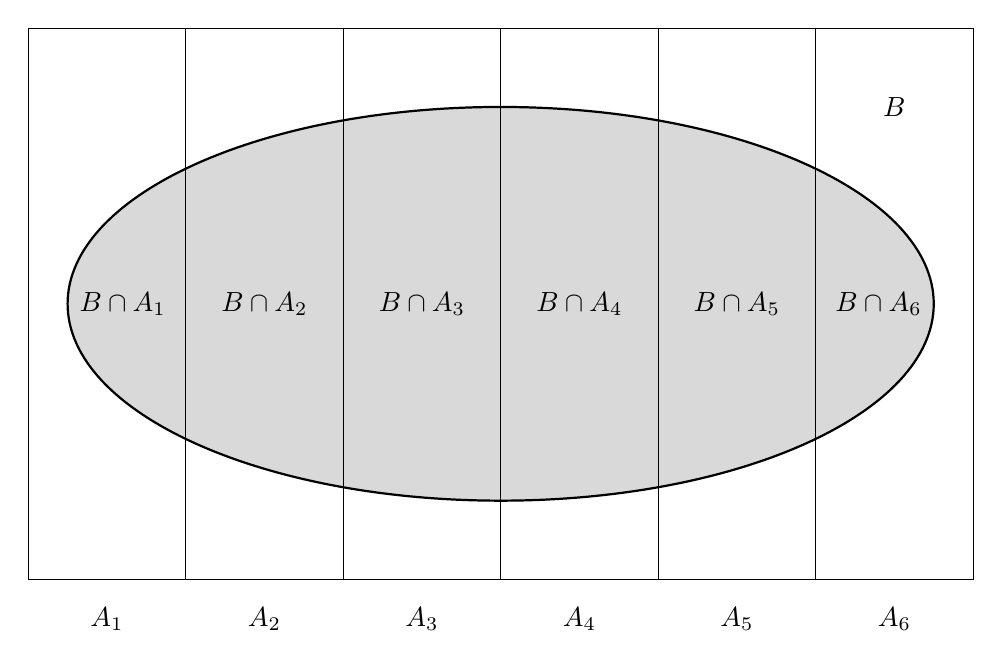
\begin{tikzpicture}
% 1. Dessiner le grand rectangle et les lignes verticales de partition
\draw (0,0) rectangle (12,7);

% 3. Dessiner une grande ellipse pour la forme B
\filldraw[
    fill=gray!30, % Remplissage gris clair
    thick % Trait épais pour le contour
] (6, 3.5) ellipse (5.5cm and 2.5cm); % Centre (6,3.5), rayon x=5.5cm, rayon y=2.5cm

\foreach \x in {2,4,6,8,10} {
    \draw (\x,0) -- (\x,7);
}

% 2. Placer les étiquettes A_1, A_2, ... en bas
\foreach \i [evaluate=\i as \xpos using \i*2-1] in {1,...,6} {
    \node at (\xpos, -0.5) {$A_{\i}$};
}

% 4. Placer l'étiquette pour l'ensemble B
\node at (11, 6) {$B$}; % Ajusté pour être au-dessus de l'ellipse

% 5. Placer les étiquettes pour les intersections B ∩ A_i, toutes au même niveau
\node at (1.2, 3.5) {$B \cap A_1$};
\node at (3, 3.5) {$B \cap A_2$};
\node at (5, 3.5) {$B \cap A_3$};
\node at (7, 3.5) {$B \cap A_4$};
\node at (9, 3.5) {$B \cap A_5$};
\node at (10.8, 3.5) {$B \cap A_6$};
\end{tikzpicture}
\end{center}
\end{intuitionbox}

\begin{examplebox}
Une usine possède trois machines, M1, M2, et M3, qui produisent respectivement 50\%, 30\% et 20\% des articles. Leurs taux de production défectueuse sont de 4\%, 2\% et 5\%. Quelle est la probabilité qu'un article choisi au hasard soit défectueux ?
Soit $D$ l'événement "l'article est défectueux". Les machines forment une partition avec $P(M1)=0.5$, $P(M2)=0.3$, et $P(M3)=0.2$. Les probabilités conditionnelles de défaut sont $P(D|M1)=0.04$, $P(D|M2)=0.02$, et $P(D|M3)=0.05$.
En appliquant la formule, on obtient :
$P(D) = P(D|M1)P(M1) + P(D|M2)P(M2) + P(D|M3)P(M3) = (0.04 \times 0.5) + (0.02 \times 0.3) + (0.05 \times 0.2) = 0.02 + 0.006 + 0.01 = 0.036$.
La probabilité qu'un article soit défectueux est de 3.6\%.
\end{examplebox}

\begin{proofbox}[Démonstration de la formule des probabilités totales]
Puisque les $A_i$ forment une partition de $S$, on peut décomposer $B$ comme :
$$B = (B \cap A_1) \cup (B \cap A_2) \cup \cdots \cup (B \cap A_n)$$
Comme les $A_i$ sont disjoints, les événements $(B \cap A_i)$ le sont aussi. On peut donc sommer leurs probabilités :
$$P(B) = P(B \cap A_1) + P(B \cap A_2) + \cdots + P(B \cap A_n)$$
En appliquant le théorème de l'intersection des probabilités à chaque terme, on obtient :
$$P(B) = P(B|A_1)P(A_1) + P(B|A_2)P(A_2) + \cdots + P(B|A_n) = \sum_{i=1}^{n} P(B|A_i)P(A_i)$$
\end{proofbox}

\subsection{Règle de Bayes avec Conditionnement Additionnel}

\begin{theorembox}[Règle de Bayes avec conditionnement additionnel]
À condition que $P(A \cap E) > 0$ et $P(B \cap E) > 0$, nous avons :
$$P(A|B, E) = \frac{P(B|A, E)P(A|E)}{P(B|E)}$$
\end{theorembox}

\begin{intuitionbox}
Cette formule est simplement la règle de Bayes standard, mais appliquée à l'intérieur d'un univers que l'on a déjà "rétréci".

Imaginez que vous recevez une information \textbf{E} qui élimine une grande partie des possibilités. C'est votre nouveau point de départ, votre monde est plus petit. Toutes les probabilités que vous calculez désormais sont relatives à ce monde restreint.

Dans ce nouveau monde, vous recevez une autre information, l'évidence \textbf{B}. La règle de Bayes conditionnelle vous permet alors de mettre à jour votre croyance sur un événement \textbf{A}, en utilisant exactement la même logique que la règle de Bayes classique, mais en vous assurant que chaque calcul reste confiné à l'intérieur des frontières de l'univers défini par \textbf{E}.
\end{intuitionbox}

\subsection{Formule des Probabilités Totales avec Conditionnement Additionnel}

\begin{theorembox}[Formule des probabilités totales avec conditionnement additionnel]
Soit $A_1, \dots, A_n$ une partition de $S$. À condition que $P(A_i \cap E) > 0$ pour tout $i$, nous avons :
$$P(B|E) = \sum_{i=1}^{n} P(B|A_i, E)P(A_i|E)$$
\end{theorembox}

\begin{intuitionbox}
\begin{center}
\begin{tikzpicture}
  % Matrice principale, nommée "m"
  \matrix (m) [
    matrix of nodes,
    row sep = -\pgflinewidth,
    column sep = -\pgflinewidth,
    nodes={
      rectangle, draw=black, anchor=center,
      text height=4ex, text depth=0.5ex, minimum width=4em, fill=intuitionColor!10
    }
  ]
  {
    | |              & | |              & |[red_hatch]|    & | |              & | |              & | |            \\
    |[red_hatch]|    & |[purple_hatch]| & |[purple_hatch]| & | |              & |[red_hatch]|    & |[red_hatch]|  \\
    |[red_hatch]|    & |[blue_hatch]|   & |[red_hatch]|    & |[red_hatch]|    & |[red_hatch]|    & | |            \\
  };

  % --- DÉLIMITATION DES COLONNES AVEC ACCOLADES ---
  \draw [decorate, decoration={brace, amplitude=5pt, raise=4mm}]
    (m-1-1.north west) -- (m-1-2.north east) 
    node [midway, yshift=8mm, font=\bfseries] {A1};
    
  \draw [decorate, decoration={brace, amplitude=5pt, raise=4mm}]
    (m-1-3.north west) -- (m-1-4.north east) 
    node [midway, yshift=8mm, font=\bfseries] {A2};
    
  \draw [decorate, decoration={brace, amplitude=5pt, raise=4mm}]
    (m-1-5.north west) -- (m-1-6.north east) 
    node [midway, yshift=8mm, font=\bfseries] {A3};
\end{tikzpicture}
\end{center}
Imaginez que le graphique ci-dessus représente la carte d'un trésor. La carte est partitionnée en trois grandes régions : \textbf{A1}, \textbf{A2}, et \textbf{A3}. Sur cette carte, on a identifié deux types de terrains : une \textbf{zone marécageuse} (événement E, hachures rouges) qui s'étend sur \textbf{10 parcelles}, et une \textbf{zone près d'un vieux chêne} (événement B, hachures bleues) qui couvre \textbf{3 parcelles}.

On vous donne un premier indice : "Le trésor est dans la zone marécageuse (E)". Votre univers de recherche se réduit instantanément à ces 10 parcelles rouges. Puis, on vous donne un second indice : "Le trésor est aussi près d'un chêne (B)". Votre recherche se concentre alors sur les parcelles qui sont à la fois marécageuses et proches d'un chêne (les cases violettes, $B \cap E$).

La question est : "Sachant que le trésor est dans une parcelle violette, quelle est la probabilité qu'il se trouve dans la région A2 ?". On cherche donc $P(A_2 | B, E)$. La règle de Bayes nous permet de le calculer.

\textbf{Calcul des termes nécessaires :} D'abord, nous devons évaluer les probabilités à l'intérieur du "monde marécageux" (sachant E).

La \textbf{vraisemblance} est $P(B|A_2, E)$. En se limitant aux 4 parcelles marécageuses de la région A2, une seule est aussi près d'un chêne. Donc, $P(B|A_2, E) = 1/4$.

La \textbf{probabilité a priori} est $P(A_2|E)$. Sur les 10 parcelles marécageuses, 4 sont dans la région A2. Donc, $P(A_2|E) = 4/10$.

L'\textbf{évidence}, $P(B|E)$, est la probabilité de trouver un chêne dans l'ensemble de la zone marécageuse. On peut la calculer avec la formule des probabilités totales :
$$P(B|E) = P(B|A_1, E)P(A_1|E) + P(B|A_2, E)P(A_2|E) + P(B|A_3, E)P(A_3|E)$$
$$P(B|E) = (\frac{1}{3} \times \frac{3}{10}) + (\frac{1}{4} \times \frac{4}{10}) + (0 \times \frac{3}{10}) = \frac{1}{10} + \frac{1}{10} = \frac{2}{10}$$

\textbf{Application de la règle de Bayes :} Maintenant, nous assemblons le tout.
$$P(A_2|B, E) = \frac{P(B|A_2, E)P(A_2|E)}{P(B|E)} = \frac{(1/4) \times (4/10)}{2/10} = \frac{1/10}{2/10} = \frac{1}{2}$$
L'intuition confirme le calcul : sachant que le trésor est sur une parcelle violette, et qu'il n'y en a que deux (une en A1, une en A2), il y a bien une chance sur deux qu'il se trouve dans la région A2.
\end{intuitionbox}

\subsection{Indépendance de Deux Événements}

\begin{definitionbox}[Indépendance de deux événements]
Les événements $A$ et $B$ sont indépendants si :
$$P(A \cap B) = P(A)P(B)$$
Si $P(A) > 0$ et $P(B) > 0$, cela est équivalent à :
$$P(A|B) = P(A)$$
\end{definitionbox}

\begin{intuitionbox}
L'indépendance est l'absence d'information. Si deux événements sont indépendants, apprendre que l'un s'est produit ne change absolument rien à la probabilité de l'autre. Savoir qu'il pleut à Tokyo ($B$) ne modifie pas la probabilité que vous obteniez pile en lançant une pièce ($A$).
\end{intuitionbox}

\subsection{Indépendance Conditionnelle}

\begin{definitionbox}[Indépendance Conditionnelle]
Les événements $A$ et $B$ sont dits conditionnellement indépendants étant donné $E$ si :
$$P(A \cap B | E) = P(A|E)P(B|E)$$
\end{definitionbox}

\begin{intuitionbox}
L'indépendance peut apparaître ou disparaître quand on observe un autre événement. Par exemple, vos notes en maths ($A$) et en physique ($B$) ne sont probablement pas indépendantes. Mais si l'on sait que vous avez beaucoup travaillé ($E$), alors vos notes en maths et en physique pourraient devenir indépendantes. L'information "vous avez beaucoup travaillé" explique la corrélation ; une fois qu'on la connaît, connaître votre note en maths n'apporte plus d'information sur votre note en physique.
\end{intuitionbox}

\subsection{Le Problème de Monty Hall}

\begin{interludebox}[Le problème de Monty Hall]
Imaginez que vous êtes à un jeu télévisé. Face à vous se trouvent trois portes fermées. Derrière l'une d'elles se trouve une voiture, et derrière les deux autres, des chèvres.
\begin{enumerate}
    \item Vous choisissez une porte (disons, la porte n°1).
    \item L'animateur, qui sait où se trouve la voiture, ouvre une autre porte (par exemple, la n°3) derrière laquelle se trouve une chèvre.
    \item Il vous demande alors : "Voulez-vous conserver votre choix initial (porte n°1) ou changer pour l'autre porte restante (la n°2) ?"
\end{enumerate}
\textbf{Question :} Avez-vous intérêt à changer de porte ? Votre probabilité de gagner la voiture est-elle plus grande si vous changez, si vous ne changez pas, ou est-elle la même dans les deux cas ?
\end{interludebox}

\begin{correctionbox}[Solution du problème de Monty Hall]
La réponse est sans équivoque : il faut \textbf{toujours changer de porte}. Cette stratégie fait passer la probabilité de gagner de $1/3$ à $2/3$. L'intuition et la preuve ci-dessous détaillent ce résultat surprenant.
\end{correctionbox}

\begin{intuitionbox}[Le secret : l'information de l'animateur]
L'erreur commune est de supposer qu'il reste deux portes avec une chance égale de $1/2$. Cela ignore une information capitale : le choix de l'animateur n'est \textbf{pas aléatoire}. Il sait où se trouve la voiture et ouvrira toujours une porte perdante.

Le raisonnement correct se déroule en deux temps. D'abord, votre choix initial a $\mathbf{1/3}$ de chance d'être correct. Cela implique qu'il y a $\mathbf{2/3}$ de chance que la voiture soit derrière l'une des \textit{deux autres portes}. Ensuite, lorsque l'animateur ouvre l'une de ces deux portes, il ne fait que vous montrer où la voiture n'est \textit{pas} dans cet ensemble. La probabilité de $2/3$ se \textbf{concentre} alors entièrement sur la seule porte qu'il a laissée fermée. Changer de porte revient à miser sur cette probabilité de $2/3$.
\end{intuitionbox}

\begin{proofbox}[Preuve par l'arbre de décision]
L'analyse de la meilleure stratégie peut être visualisée à l'aide de l'arbre de décision ci-dessous. Il décompose le problème en deux scénarios initiaux : avoir choisi la bonne porte (probabilité $1/3$) ou une mauvaise porte (probabilité $2/3$).

\vspace{0.5cm}
\begin{center}
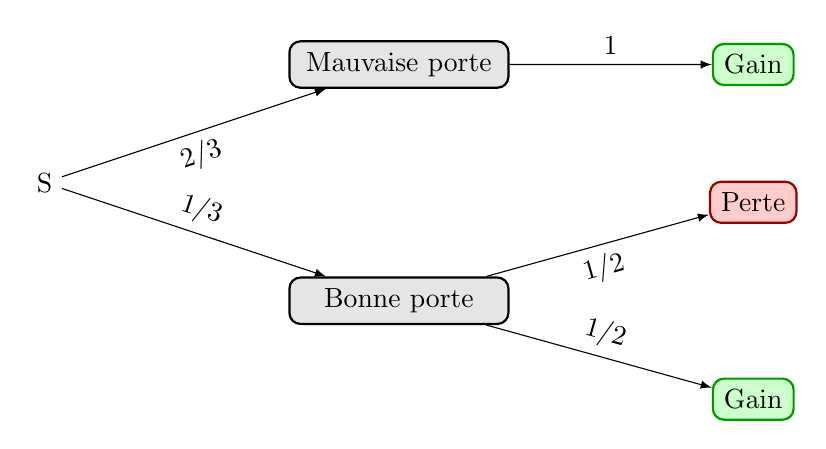
\begin{tikzpicture}[
  grow=right,
  level distance=4.5cm,
  level 1/.style={sibling distance=3cm},
  level 2/.style={sibling distance=2.5cm},
  edge from parent/.style={draw, -latex},
  % --- Définition des styles pour les cadres ---
  porte_style/.style={rectangle, rounded corners, draw=black, fill=gray!20, thick, inner sep=4pt, text width=2.5cm, align=center},
  gain_style/.style={rectangle, rounded corners, draw=green!60!black, fill=green!20, thick, inner sep=4pt},
  perte_style/.style={rectangle, rounded corners, draw=red!60!black, fill=red!20, thick, inner sep=4pt}
]

\node {S}
    % --- Branche du haut ---
    child {
        node[porte_style] {Bonne porte}
        child {
            node[gain_style] {Gain}
            edge from parent
            node[above, sloped] {$1/2$}
        }
        child {
            node[perte_style] {Perte}
            edge from parent
            node[below, sloped] {$1/2$}
        }
        edge from parent
        node[above, sloped] {1/3}
    }
    % --- Branche du bas ---
    child {
        node[porte_style] {Mauvaise porte}
        child {
            node[gain_style] {Gain}
            edge from parent
            node[above, sloped] {1}
        }
        edge from parent
        node[below, sloped] {2/3}
    };
\end{tikzpicture}
\end{center}
\vspace{0.5cm}

\noindent\textbf{Analyse de l'arbre :}

\vspace{0.3cm}
\noindent\textbf{Branche du bas (cas le plus probable) :}
\newline
Avec une probabilité de $\mathbf{2/3}$, votre choix initial se porte sur une "Mauvaise porte". L'animateur est alors obligé de révéler l'autre porte perdante. La seule porte restante est donc la bonne. L'arbre montre que cela mène à un "Gain" avec une probabilité de $\mathbf{1}$. Ce chemin correspond au résultat de la stratégie \textbf{"Changer"}.

\vspace{0.3cm}
\noindent\textbf{Branche du haut (cas le moins probable) :}
\newline
Avec une probabilité de $\mathbf{1/3}$, vous avez choisi la "Bonne porte" du premier coup. L'arbre se divise alors en deux issues équiprobables ($1/2$ chacune). L'issue "Gain" correspond à la stratégie \textbf{"Garder"} votre choix initial, tandis que l'issue "Perte" correspond à la stratégie \textbf{"Changer"} pour la porte perdante restante.

\vspace{0.3cm}
\noindent\textbf{Conclusion :}
\newline
Pour évaluer la meilleure stratégie, il suffit de sommer les probabilités de gain. La \textbf{probabilité de gain en changeant} est de $\mathbf{2/3}$, car vous gagnez uniquement si votre choix initial était mauvais (branche du bas). La \textbf{probabilité de gain en gardant} est de $\mathbf{1/3}$, car vous gagnez uniquement si votre choix initial était bon (branche "Gain" du haut). La stratégie optimale est donc bien de toujours changer de porte.
\end{proofbox}